% =====================================================================
%  Informe de práctica de laboratorio (formato UMNG) – Robot móvil ESP32
%  Compilar:  cd docs/informe_umng && python3 figuras.py && pdflatex informe && pdflatex informe
% =====================================================================
\documentclass[10pt,a4paper,twocolumn]{article}
\usepackage[utf8]{inputenc}
\usepackage[T1]{fontenc}
\usepackage[spanish,es-tabla,es-nodecimaldot]{babel}
\usepackage{mathptmx}
\usepackage[a4paper,top=2.7cm,bottom=2.2cm,left=1.7cm,right=1.7cm,headheight=1.3cm,headsep=0.6cm,
            columnsep=0.75cm]{geometry}
\usepackage{graphicx,booktabs,array,tabularx,multirow,amsmath,amssymb,xcolor,listings,enumitem}
\usepackage{fancyhdr,titlesec,caption,url}
\usepackage[hidelinks]{hyperref}

% ------------------------------------------------------------- encabezado
\pagestyle{fancy}
\fancyhf{}
\fancyhead[L]{\raisebox{-0.35\height}{
\includegraphics[height=0.95cm]{fig/logo_umng.png}}}
\fancyhead[C]{\footnotesize INFORME DE PRÁCTICA DE LABORATORIO\\PROGRAMA DE INGENIERÍA MECATRÓNICA}
\fancyhead[R]{\footnotesize Versión 1.0\\Periodo 2026-2}
\fancyfoot[C]{\thepage}
\renewcommand{\headrulewidth}{0pt}
\fancypagestyle{plain}{\fancyhf{}%
  \fancyhead[L]{\raisebox{-0.35\height}{
\includegraphics[height=0.95cm]{fig/logo_umng.png}}}%
  \fancyhead[C]{\footnotesize INFORME DE PRÁCTICA DE LABORATORIO\\PROGRAMA DE INGENIERÍA MECATRÓNICA}%
  \fancyhead[R]{\footnotesize Versión 1.0\\Periodo 2026-2}\fancyfoot[C]{\thepage}%
  \renewcommand{\headrulewidth}{0pt}}

% ------------------------------------------------------------- títulos de sección (estilo IEEE)
\renewcommand{\thesection}{\Roman{section}}
\renewcommand{\thesubsection}{\Alph{subsection}}
\titleformat{\section}{\centering\normalsize\scshape}{\thesection.}{0.5em}{}
\titlespacing*{\section}{0pt}{1.4ex}{0.9ex}
\titleformat{\subsection}{\normalsize\itshape}{\thesubsection.}{0.5em}{}
\titlespacing*{\subsection}{0pt}{1.1ex}{0.5ex}
\captionsetup{font=small,labelsep=colon}
\captionsetup[table]{position=top,skip=3pt}
\setlength{\parindent}{1em}
\setlist{nosep,leftmargin=1.2em}
\renewcommand{\arraystretch}{1.12}

% ------------------------------------------------------------- código
\definecolor{cmt}{RGB}{90,110,90}
\lstset{language=C++,basicstyle=\ttfamily\scriptsize,columns=fullflexible,breaklines=true,
  commentstyle=\color{cmt}\itshape,keywordstyle=\bfseries,showstringspaces=false,frame=none,
  literate={á}{{\'a}}1 {é}{{\'e}}1 {í}{{\'i}}1 {ó}{{\'o}}1 {ú}{{\'u}}1 {ñ}{{\~n}}1
           {Á}{{\'A}}1 {É}{{\'E}}1 {Í}{{\'I}}1 {Ó}{{\'O}}1 {Ú}{{\'U}}1 {°}{{$^\circ$}}1 {–}{{--}}1}

\newcommand{\ra}{$\rightarrow$}

\begin{document}

\twocolumn[{%
\begin{center}
  \vspace*{0.3cm}
  {\LARGE ROBOT MÓVIL AUTÓNOMO CON ESP32: SEGUIDOR DE LÍNEA CON BRÚJULA DIGITAL, DETECCIÓN DE COLORES Y EVASIÓN DE OBSTÁCULOS\,\footnotemark}\\[0.45cm]
  {\large Escobar Jaramillo Ana Sofía (7004641), Moreno Lina María (7004589)}\\[0.6cm]
\end{center}}]
\footnotetext{El presente documento corresponde al primer entregable (corte 2) del proyecto final, presentado en la Universidad Militar Nueva Granada durante el periodo 2026-2.}

\noindent\textbf{\textit{Resumen}— El proyecto tiene como propósito diseñar e implementar un robot móvil basado en ESP32, con estructura mecánica y electrónica propias, que opere en modo manual (comandos de voz desde una aplicación Streamlit y un control remoto construido con un segundo ESP32) y en modo autónomo. En modo autónomo el robot sigue una línea guía con tres sensores infrarrojos, mantiene el rumbo con una brújula digital QMC5883L, detecta seis colores de la superficie con un sensor TCS34725 y esquiva obstáculos con un ultrasonido HC-SR04 montado sobre un servomotor, retomando la pista en el sentido original. Un termistor NTC protege el paquete de baterías y una API REST sobre Wi-Fi alimenta un tablero en tiempo real con la dirección polar actual y deseada, y un chatbot tipo J.A.R.V.I.S. que explica el proyecto y las variables medidas. La lógica de control se validó en un gemelo digital que expone la misma API del firmware: en pistas dibujadas sobre 1, 2, 4 y 6 pliegos, con 0, 4, 6 y 8 obstáculos, el robot completó 5 minutos de recorrido continuo sin colisiones.}

\vspace{0.2cm}
\noindent\textbf{\textit{Abstract}— \textit{This project aims to design and implement an ESP32-based mobile robot, with its own mechanical and electronic design, able to operate in manual mode (voice commands from a Streamlit application and a remote control built with a second ESP32) and in autonomous mode. In autonomous mode the robot follows a guide line with three infrared sensors, holds its heading with a QMC5883L digital compass, detects six surface colours with a TCS34725 sensor and avoids obstacles with an HC-SR04 ultrasonic sensor mounted on a servo, returning to the track in its original direction. An NTC thermistor protects the battery pack, and a REST API over Wi-Fi feeds a real-time dashboard showing the current and desired polar heading, and a J.A.R.V.I.S.-like chatbot that explains the project and the measured variables. The control logic was validated in a digital twin exposing the same API as the firmware: on tracks drawn on 1, 2, 4 and 6 paper sheets with 0, 4, 6 and 8 obstacles, the robot ran continuously for 5 minutes without collisions.}}

\vspace{0.2cm}
\noindent\textbf{\textit{Palabras clave}— Robot móvil, ESP32, seguidor de línea, brújula digital, TCS34725, evasión de obstáculos, termistor NTC, Streamlit, ESP-NOW, gemelo digital.}

\section{Introducción}
Los robots móviles de tracción diferencial son la plataforma más usada para enseñar percepción, control y comunicación inalámbrica, porque con dos motores y pocos sensores permiten implementar navegación completa. Un seguidor de línea resuelve la localización con sensores de reflexión; añadir una brújula permite mantener el rumbo cuando la línea se pierde, y un sensor de distancia permite reaccionar a obstáculos.

La guía del proyecto pide un sistema robótico móvil basado en ESP32 que opere en modo manual (voz y control propio con ESP32) y autónomo, se oriente con una brújula digital, se comunique de forma inalámbrica con una aplicación Streamlit que muestre en tiempo real la dirección polar actual y deseada, detecte cambios de color de la superficie (negro, blanco, rojo, amarillo, verde y azul) y obstáculos (esquivándolos y siguiendo el trayecto) e incorpore un chatbot tipo J.A.R.V.I.S. La meta final son tres pistas con 4, 6 y 8 obstáculos y 3, 4 y 6 colores.

Este primer entregable cubre los cuatro objetivos específicos del corte 2: arquitectura y requerimientos, diseño mecánico y electrónico, construcción de los módulos y desarrollo de la aplicación. El firmware se verificó en un gemelo digital; las pruebas sobre el robot físico se realizan durante el montaje con un programa de pruebas por módulo (Sección~VI-\ref{sec:montaje}).

\section{Marco teórico}
\textbf{Cinemática diferencial.} Con velocidades de rueda $v_L$ y $v_R$ y ancho de vía $b$, la velocidad lineal y angular del robot son
\begin{equation}
v=\frac{v_R+v_L}{2},\qquad \omega=\frac{v_R-v_L}{b}.
\end{equation}
El control se expresa como avance $v^\ast$ y giro $w^\ast$ normalizados y se mezcla en $u_L=v^\ast+w^\ast$, $u_R=v^\ast-w^\ast$, reescalando si $\max(|u_L|,|u_R|)>1$.

\textbf{Seguimiento de línea.} Tres sensores de reflexión infrarroja (izquierda, centro, derecha) dan valores binarios $l,c,r$. El error lateral es $e=(r-l)/(l+c+r)\in[-1,1]$ y un control proporcional aplica $w^\ast=K_l\,e$.

\textbf{Brújula digital.} El magnetómetro mide las componentes $(m_x,m_y)$ del campo. Tras corregir la distorsión por hierro duro (offset) y blando (escala),
\begin{equation}
\hat m_i=(m_i-o_i)\,s_i,\quad o_i=\frac{m_{i,\max}+m_{i,\min}}{2},\quad s_i=\frac{\bar r}{r_i},
\end{equation}
el rumbo es $\psi=\operatorname{atan2}(\hat m_y,\hat m_x)+\delta$, con $\delta$ la declinación magnética local. El error de rumbo se normaliza a $[-180^\circ,180^\circ)$ para que el robot gire siempre por el lado más corto.

\textbf{Detección de color.} El TCS34725 entrega cuatro canales de 16 bits ($R,G,B,C$). La cromaticidad normalizada
\begin{equation}
\tilde r=\frac{R}{R+G+B},\quad \tilde g=\frac{G}{R+G+B},\quad \tilde b=\frac{B}{R+G+B}
\end{equation}
separa el tono de la intensidad; el brillo $\log_{10}C$ distingue negro de blanco. Cada lectura se asigna a la referencia más cercana.

\textbf{Ultrasonido.} La distancia se obtiene del tiempo de vuelo del eco, $d=v_s\,t/2$, con $v_s\approx343$\,m/s.

\textbf{Divisor de tensión y termistor.} Un divisor entrega $V_o=V_i\,R_2/(R_1+R_2)$. La resistencia de un termistor NTC sigue el modelo Beta
\begin{equation}
\frac{1}{T}=\frac{1}{T_0}+\frac{1}{\beta}\ln\frac{R}{R_0},
\end{equation}
con $T_0=298{,}15$\,K, $R_0=10$\,k$\Omega$ y $\beta=3950$\,K.

\textbf{Puente H y PWM.} El TB6612FNG controla dos canales con transistores MOSFET; el sentido lo fijan dos entradas lógicas y la magnitud un PWM. Su caída de tensión ($\approx0{,}2$\,V) es mucho menor que la de un L298N ($\approx2$\,V).

\textbf{Comunicación.} El ESP32 crea un punto de acceso Wi-Fi (SoftAP) y atiende peticiones HTTP con respuestas JSON (API REST). ESP-NOW permite enviar paquetes cortos entre ESP32 sin router, con latencia de pocos milisegundos.

\section{Materiales y métodos}
\subsection{Materiales}
En la Tabla~\ref{tab:materiales} se presentan los componentes del prototipo. Se usó el entorno Arduino para ESP32 (núcleo $\geq3.0$) con las bibliotecas \texttt{WiFi}, \texttt{WebServer}, \texttt{Wire}, \texttt{Preferences} y \texttt{esp\_now}; la aplicación, el simulador y las pruebas automáticas se hicieron en Python (Streamlit, Plotly, pytest), el modelo 3D en OpenSCAD y el chatbot con la API de Claude (Anthropic).

\begin{table}[!t]
\caption{Componentes del prototipo y su función}\label{tab:materiales}
\centering\scriptsize
\begin{tabularx}{\columnwidth}{@{}>{\raggedright\arraybackslash}p{3.3cm}>{\raggedright\arraybackslash}X@{}}
\toprule
\textbf{Componente} & \textbf{Función en el sistema}\\
\midrule
ESP32 DevKit V1 (WROOM) & Control a 20\,Hz, API REST, ESP-NOW.\\
Puente H TB6612FNG & Sentido y velocidad de los motores.\\
Motorreductores TT 1:48 + ruedas 65\,mm & Tracción diferencial.\\
GY-271 (QMC5883L) & Brújula digital (I$^2$C 0x0D).\\
TCS34725 con LED & Color de la superficie (I$^2$C 0x29).\\
HC-SR04 + servo SG90 & Distancia al obstáculo y escaneo lateral.\\
3$\times$ TCRT5000 con comparador & Línea guía.\\
Termistor NTC 10\,k B3950 & Temperatura de las baterías.\\
2$\times$ 18650 + BMS 2S & Alimentación 7,4\,V protegida.\\
Regulador MP1584 & 7,4\,V\ra5\,V, 3\,A para la lógica.\\
Fusible 3\,A, interruptor, 2$\times$470\,µF & Protección y desacople.\\
Resistencias 100k, 33k, 10k, 2k, 1k & Divisores (batería, ECHO, NTC).\\
MDF/acrílico 3\,mm, piezas PLA & Chasis de dos niveles y soportes.\\
ESP32 + joystick KY-023 & Control remoto propio (ESP-NOW).\\
Computador y multímetro & Programación y verificación.\\
\bottomrule
\end{tabularx}
\end{table}

\subsection{Métodos}
El trabajo se dividió en seis etapas:
\begin{enumerate}
\item \textbf{Requerimientos y arquitectura:} requerimientos funcionales y no funcionales, diagramas de bloques por módulo y selección justificada de materiales.
\item \textbf{Diseño mecánico:} chasis paramétrico en OpenSCAD con planos para corte láser y piezas impresas.
\item \textbf{Diseño electrónico:} etapa de potencia, asignación de pines y cálculo de divisores y consumo.
\item \textbf{Firmware modular:} un archivo por módulo y una máquina de estados para el modo autónomo.
\item \textbf{Aplicación y chatbot:} tablero Streamlit, comandos de voz y J.A.R.V.I.S.
\item \textbf{Validación:} gemelo digital con la misma API, 31 pruebas automáticas y diseño de pistas sobre pliegos validadas en simulación.
\end{enumerate}

\section{Competencias a desarrollar}
\begin{itemize}
\item Analizar requerimientos y traducirlos en una arquitectura de módulos.
\item Seleccionar sensores y actuadores con criterios técnicos y de costo.
\item Diseñar la estructura mecánica y el sistema electrónico de un robot móvil.
\item Programar un microcontrolador con lazos de control en tiempo real y máquinas de estados.
\item Calibrar sensores (magnetómetro, color, reflexión, ultrasonido, termistor).
\item Implementar comunicación inalámbrica (Wi-Fi, HTTP/JSON, ESP-NOW).
\item Desarrollar interfaces de usuario con visualización en tiempo real y voz.
\item Validar algoritmos con simulación antes de probarlos en hardware.
\end{itemize}

\section{Trabajo previo}
Antes del montaje se compararon alternativas para cada módulo. El L298N se descartó por su caída de unos 2\,V, que con una batería de 7,4\,V deja poco voltaje a los motores; se adoptó el TB6612FNG. El HMC5883L está descontinuado y los módulos GY-271 actuales traen el QMC5883L, cuyo registro se programó directamente. Para el color se prefirió el TCS34725 al TCS3200 por su salida digital con filtro IR y LED propio.

Al agregar el termistor se encontró que todos los pines del ADC1 estaban ocupados y que el ADC2 no puede leerse con el Wi-Fi activo; por eso la entrada BIN1 del puente H se movió de GPIO33 a GPIO16 y el NTC quedó en GPIO33 (ADC1).

También se construyó un gemelo digital del robot que expone la misma API HTTP del firmware y ejecuta la misma máquina de estados, y un programa de pruebas por módulo con menú serie para el montaje.

\section{Desarrollo de la práctica}
\subsection{Arquitectura del sistema}
La arquitectura es centralizada en el ESP32 (Fig.~\ref{fig:arq}), que ejecuta un lazo de percepción--decisión--actuación a 20\,Hz y atiende en paralelo la API HTTP y el receptor ESP-NOW. La potencia se separa en dos dominios: motores a 7,4\,V y lógica a 5\,V/3,3\,V, para que el ruido de los motores no reinicie el microcontrolador. Los requerimientos principales se resumen en la Tabla~\ref{tab:req}.

\begin{figure*}[!t]
\centering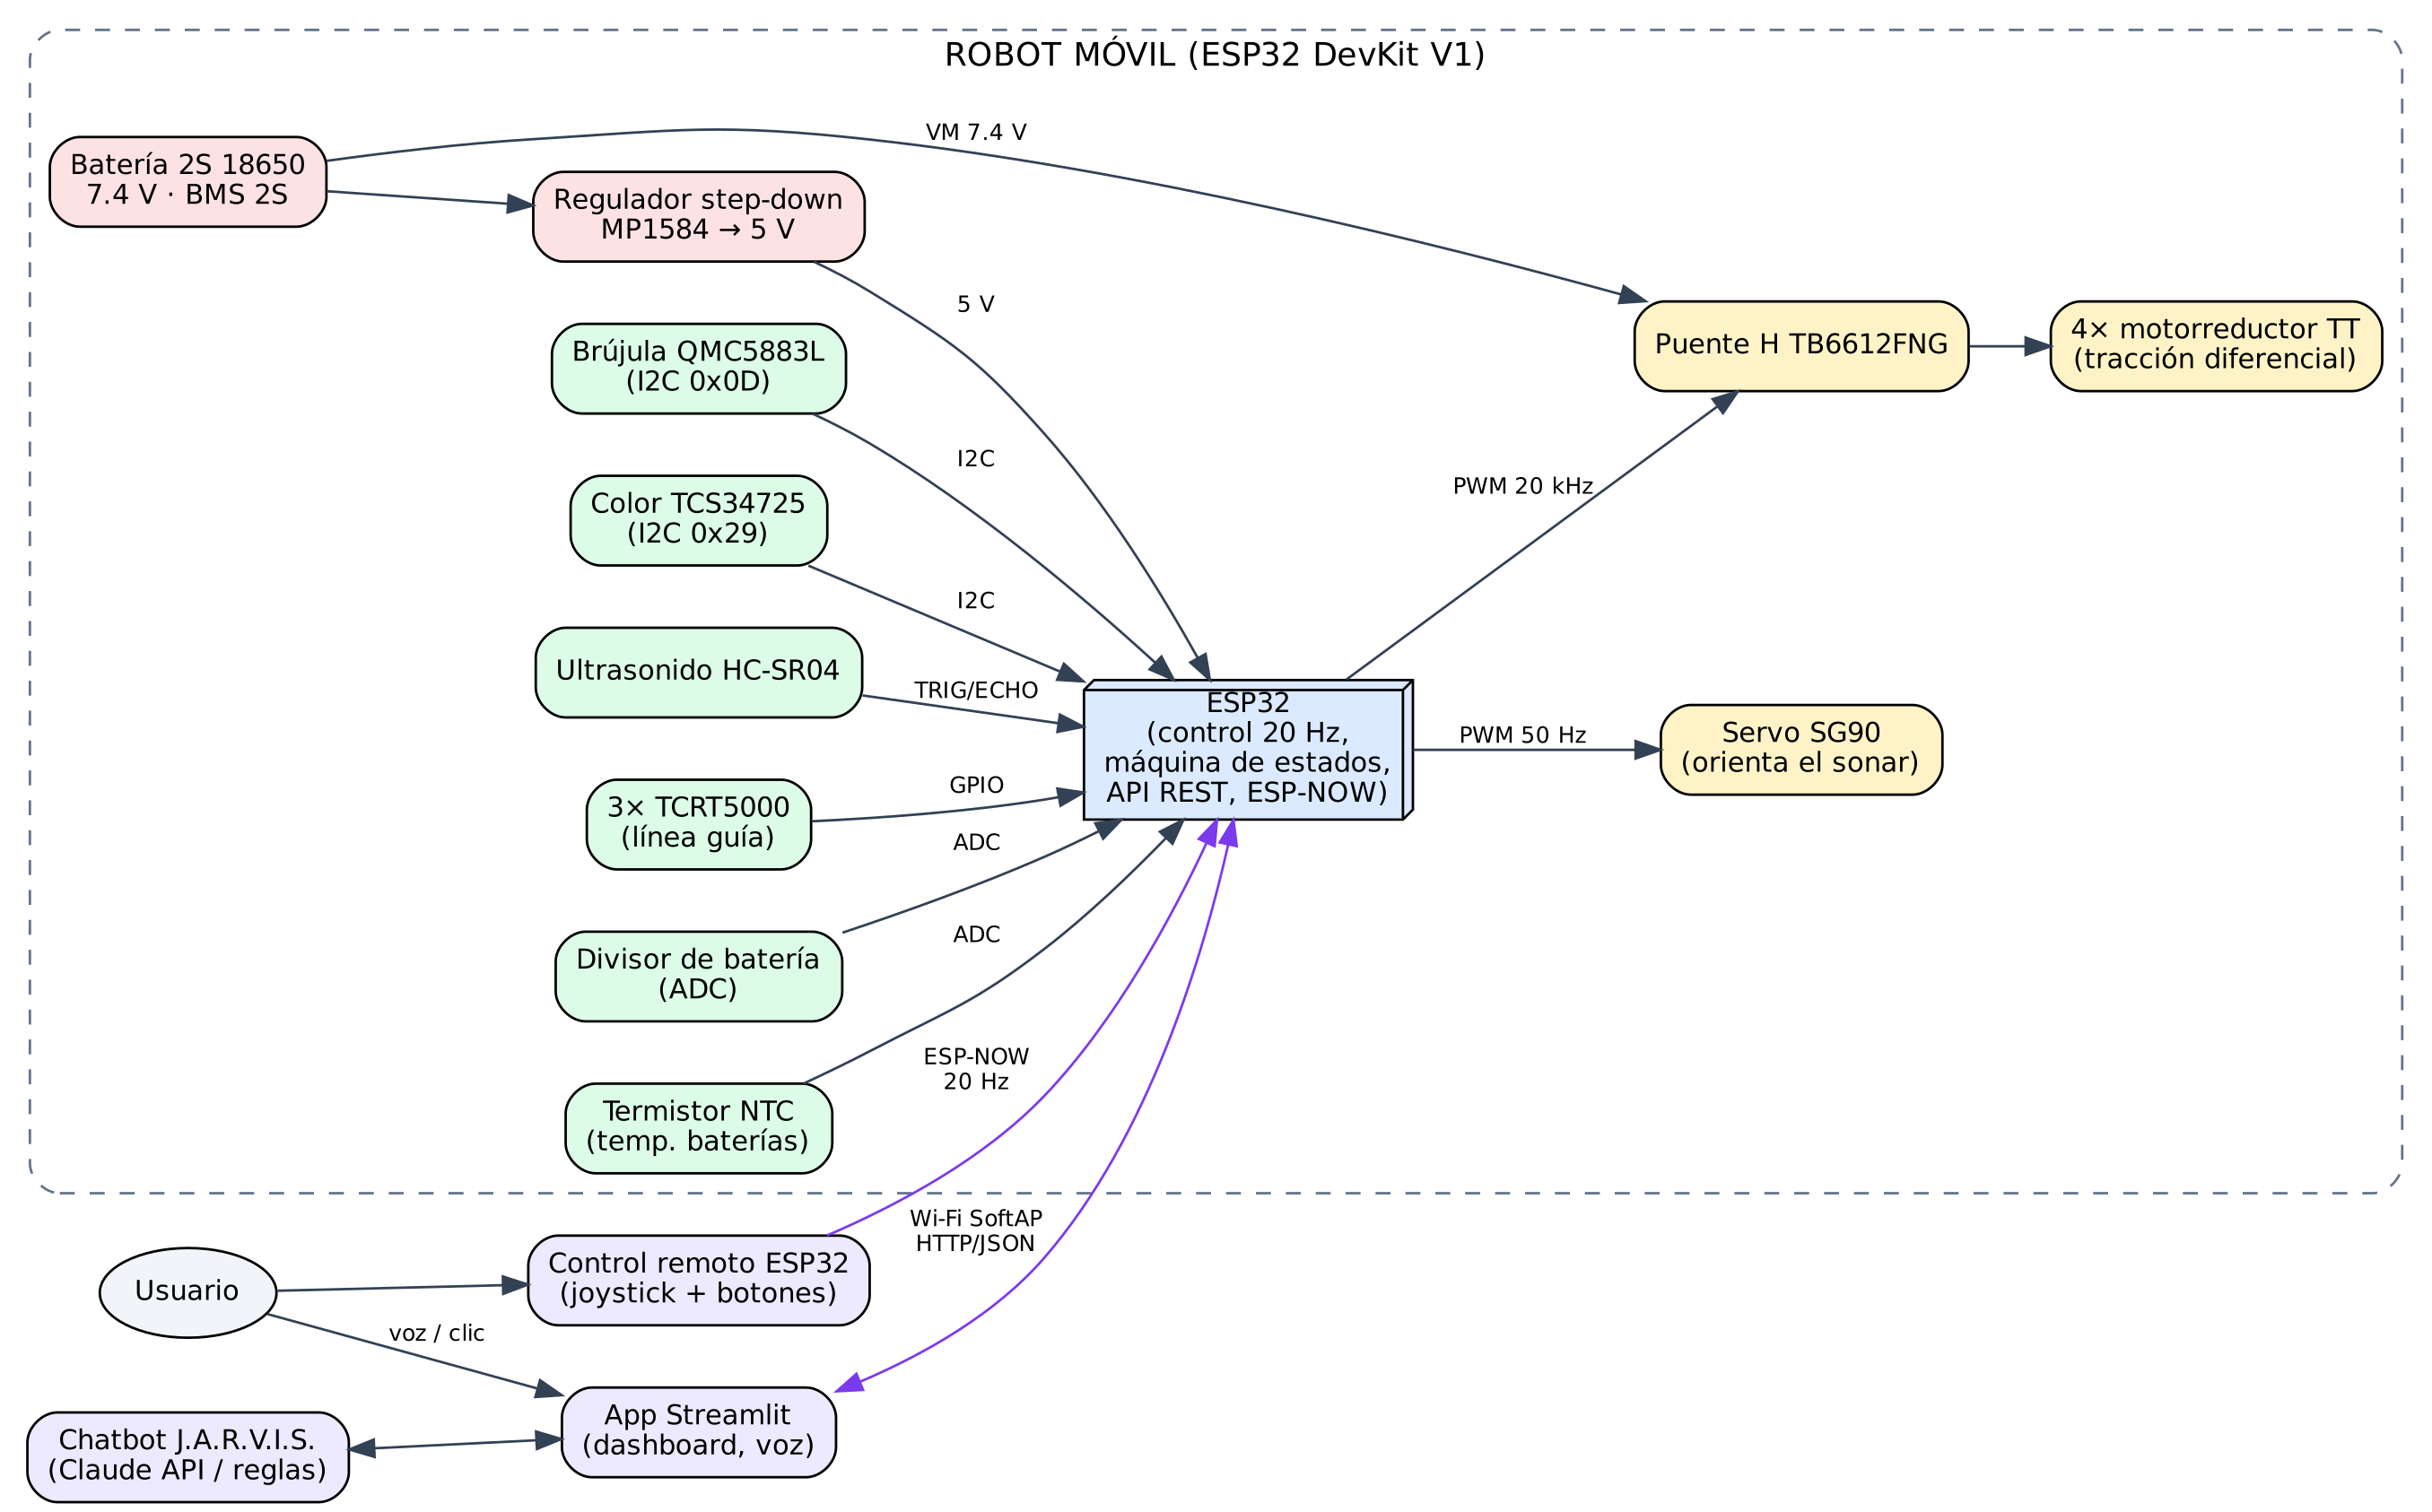
\includegraphics[width=0.92\textwidth]{fig/arquitectura_general.png}
\caption{Arquitectura general del sistema.}\label{fig:arq}
\end{figure*}

\begin{table}[!t]
\caption{Requerimientos principales}\label{tab:req}
\centering\scriptsize
\begin{tabularx}{\columnwidth}{@{}l>{\raggedright\arraybackslash}X@{}}
\toprule
\textbf{ID} & \textbf{Requerimiento}\\
\midrule
RF-01 & Moverse adelante, atrás y girar con velocidad regulable.\\
RF-02 & Comandos de voz en español (arriba, abajo, derecha, izquierda, detente).\\
RF-03 & Control remoto propio con ESP32 (ESP-NOW).\\
RF-04 & Rumbo magnético 0--360$^\circ$ con brújula calibrable.\\
RF-05 & Seguir la pista y mantener una dirección deseada.\\
RF-06 & Detectar 6 colores y los cambios de sección.\\
RF-07 & Esquivar obstáculos a menos de 30\,cm y retomar la pista.\\
RF-08 & Mostrar en la app la dirección polar actual y deseada.\\
RF-09 & Chatbot que explique el proyecto y las variables.\\
RNF-01 & Lazo de control a 20\,Hz; comando\ra motor $<150$\,ms.\\
RNF-02 & Parada si no llegan comandos (600\,ms app, 300\,ms ESP-NOW).\\
RNF-03 & Protección térmica de baterías (45\,°C aviso, 55\,°C corte).\\
RNF-04 & Autonomía $\geq45$\,min; costo $\leq450.000$\,COP.\\
\bottomrule
\end{tabularx}
\end{table}

\subsection{Diseño mecánico}
El chasis de diseño propio (Fig.~\ref{fig:cad}) tiene dos niveles de $200\times140$\,mm unidos por separadores M3 de 45\,mm: el inferior aloja motores, batería, puente H y regulador (centro de gravedad bajo) y el superior el ESP32, el servo con el ultrasonido y la brújula. Las decisiones principales fueron:
\begin{itemize}
\item \textbf{Brújula en un mástil de PLA de 80\,mm}, a unos 125\,mm de los imanes de los motores y con tornillería no ferromagnética.
\item \textbf{Sensor de color a 5\,mm del piso} dentro de un faldón que bloquea la luz ambiente, y TCRT5000 a 8\,mm.
\item \textbf{Ultrasonido a 110\,mm} sobre el servo, por encima de las ruedas, para escanear $\pm70^\circ$ sin detectar el piso.
\end{itemize}
Los planos de corte láser (DXF), las piezas impresas (STL) y la vista lateral con alturas (Fig.~\ref{fig:lateral}) se generan desde el mismo modelo paramétrico. Para probar los módulos mientras se fabrica este chasis se usa un chasis acrílico de dos motores; la lógica de control es la misma porque ambos son de tracción diferencial.

\begin{figure}[!t]
\centering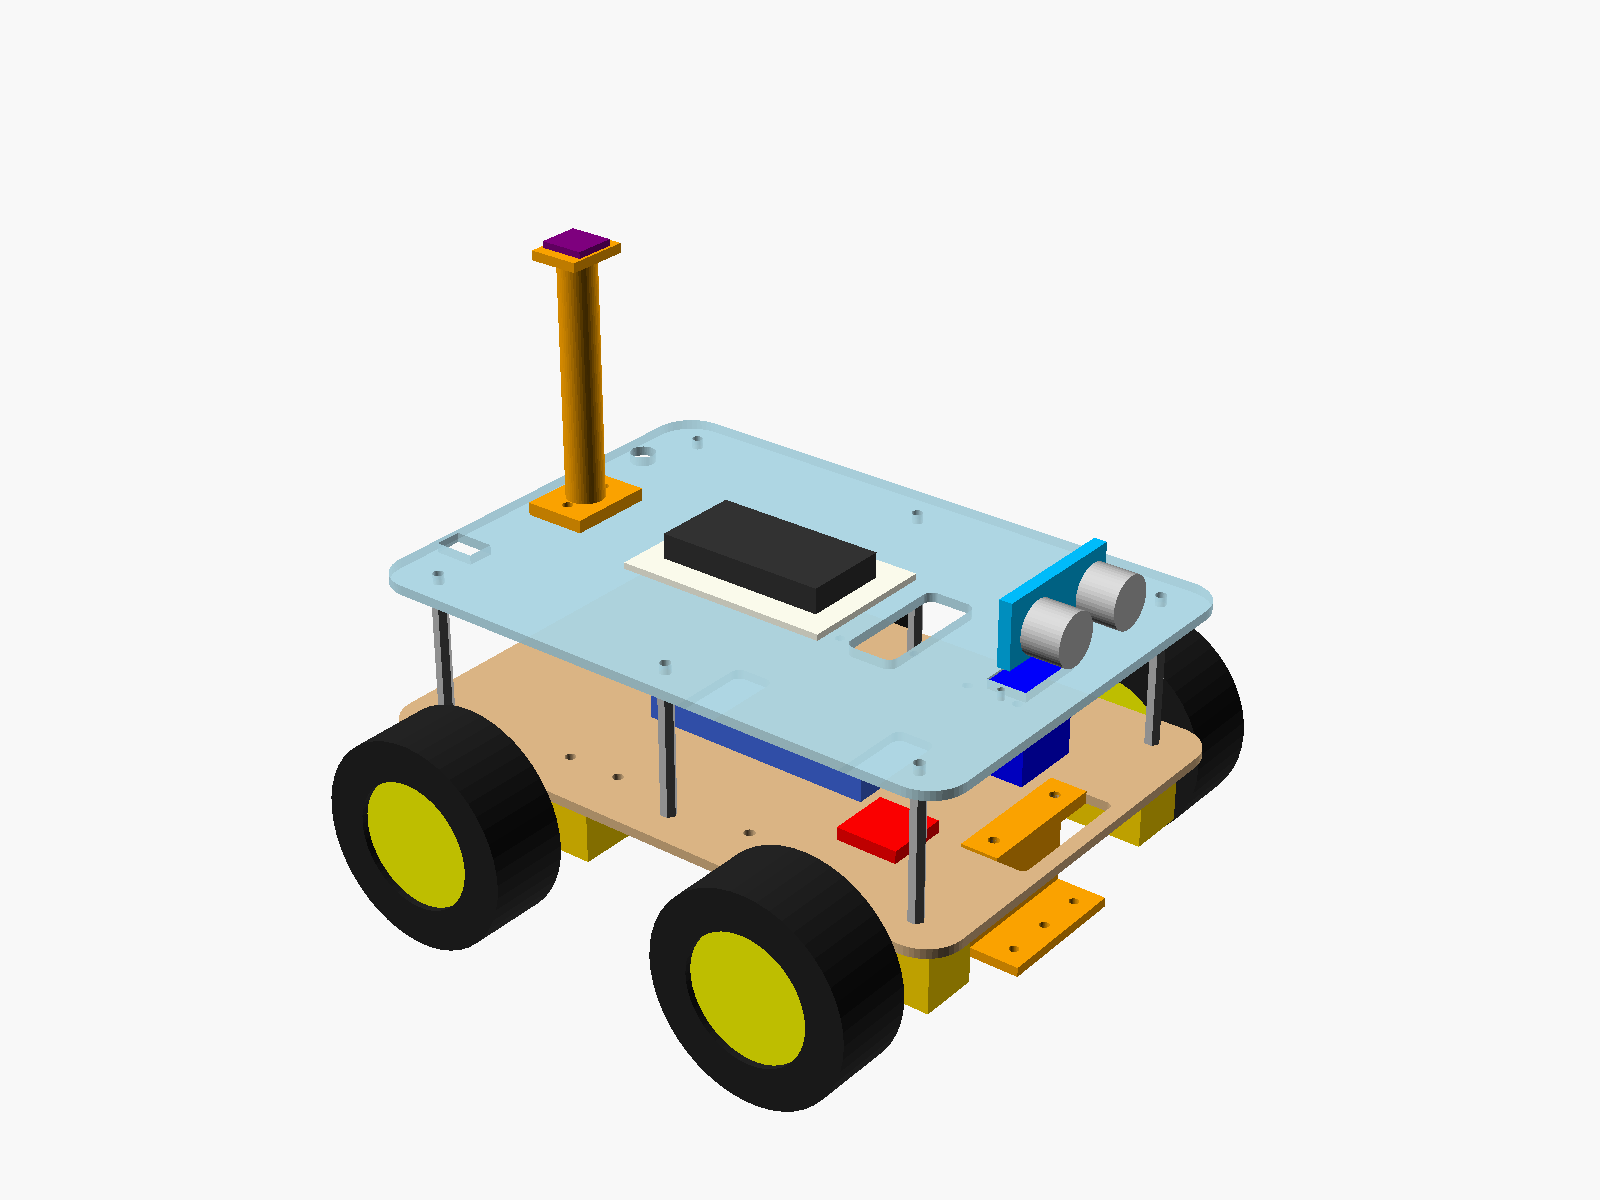
\includegraphics[width=0.78\columnwidth]{fig/render_iso.png}
\caption{Modelo CAD del chasis de dos niveles.}\label{fig:cad}
\end{figure}

\begin{figure}[!t]
\centering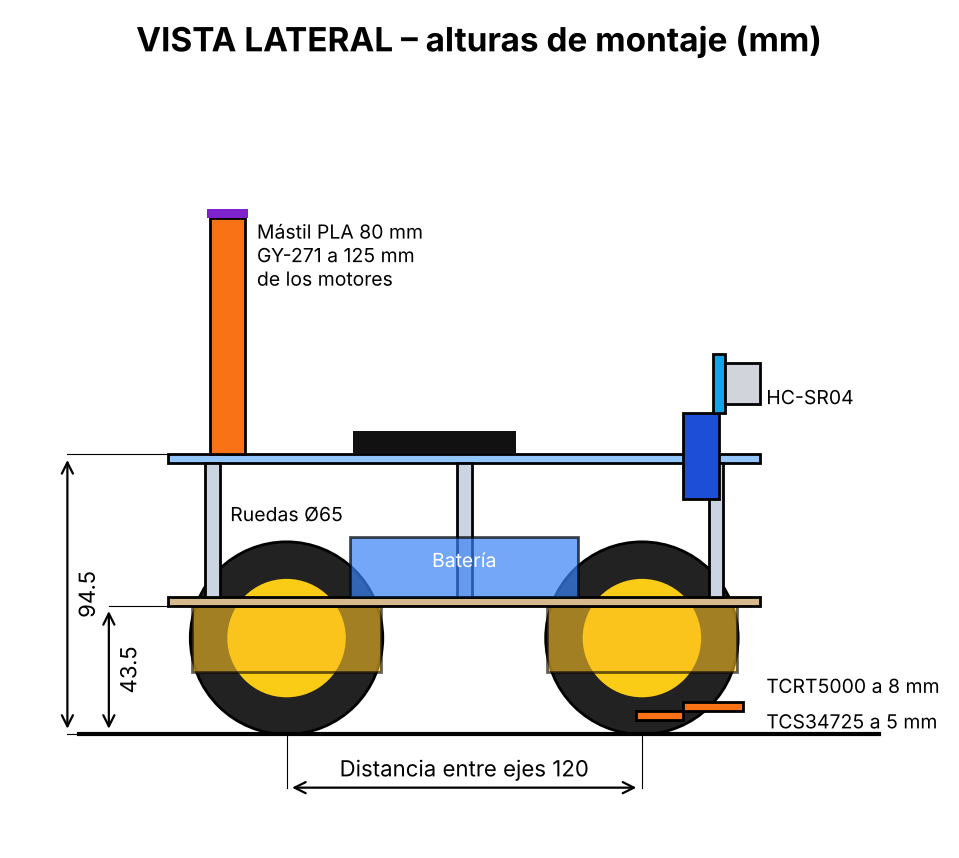
\includegraphics[width=\columnwidth]{fig/plano_lateral.png}
\caption{Vista lateral con las alturas de montaje de los sensores.}\label{fig:lateral}
\end{figure}

\subsection{Diseño electrónico}
La Fig.~\ref{fig:pot} muestra la etapa de potencia y los divisores, y la Tabla~\ref{tab:pines} la asignación de pines (esquema completo en la Fig.~\ref{fig:nets}). Se evitaron los pines de arranque (GPIO0, 12 y 15) y los sensores digitales de línea usan los pines solo-entrada 34--39.

\begin{figure*}[!t]
\centering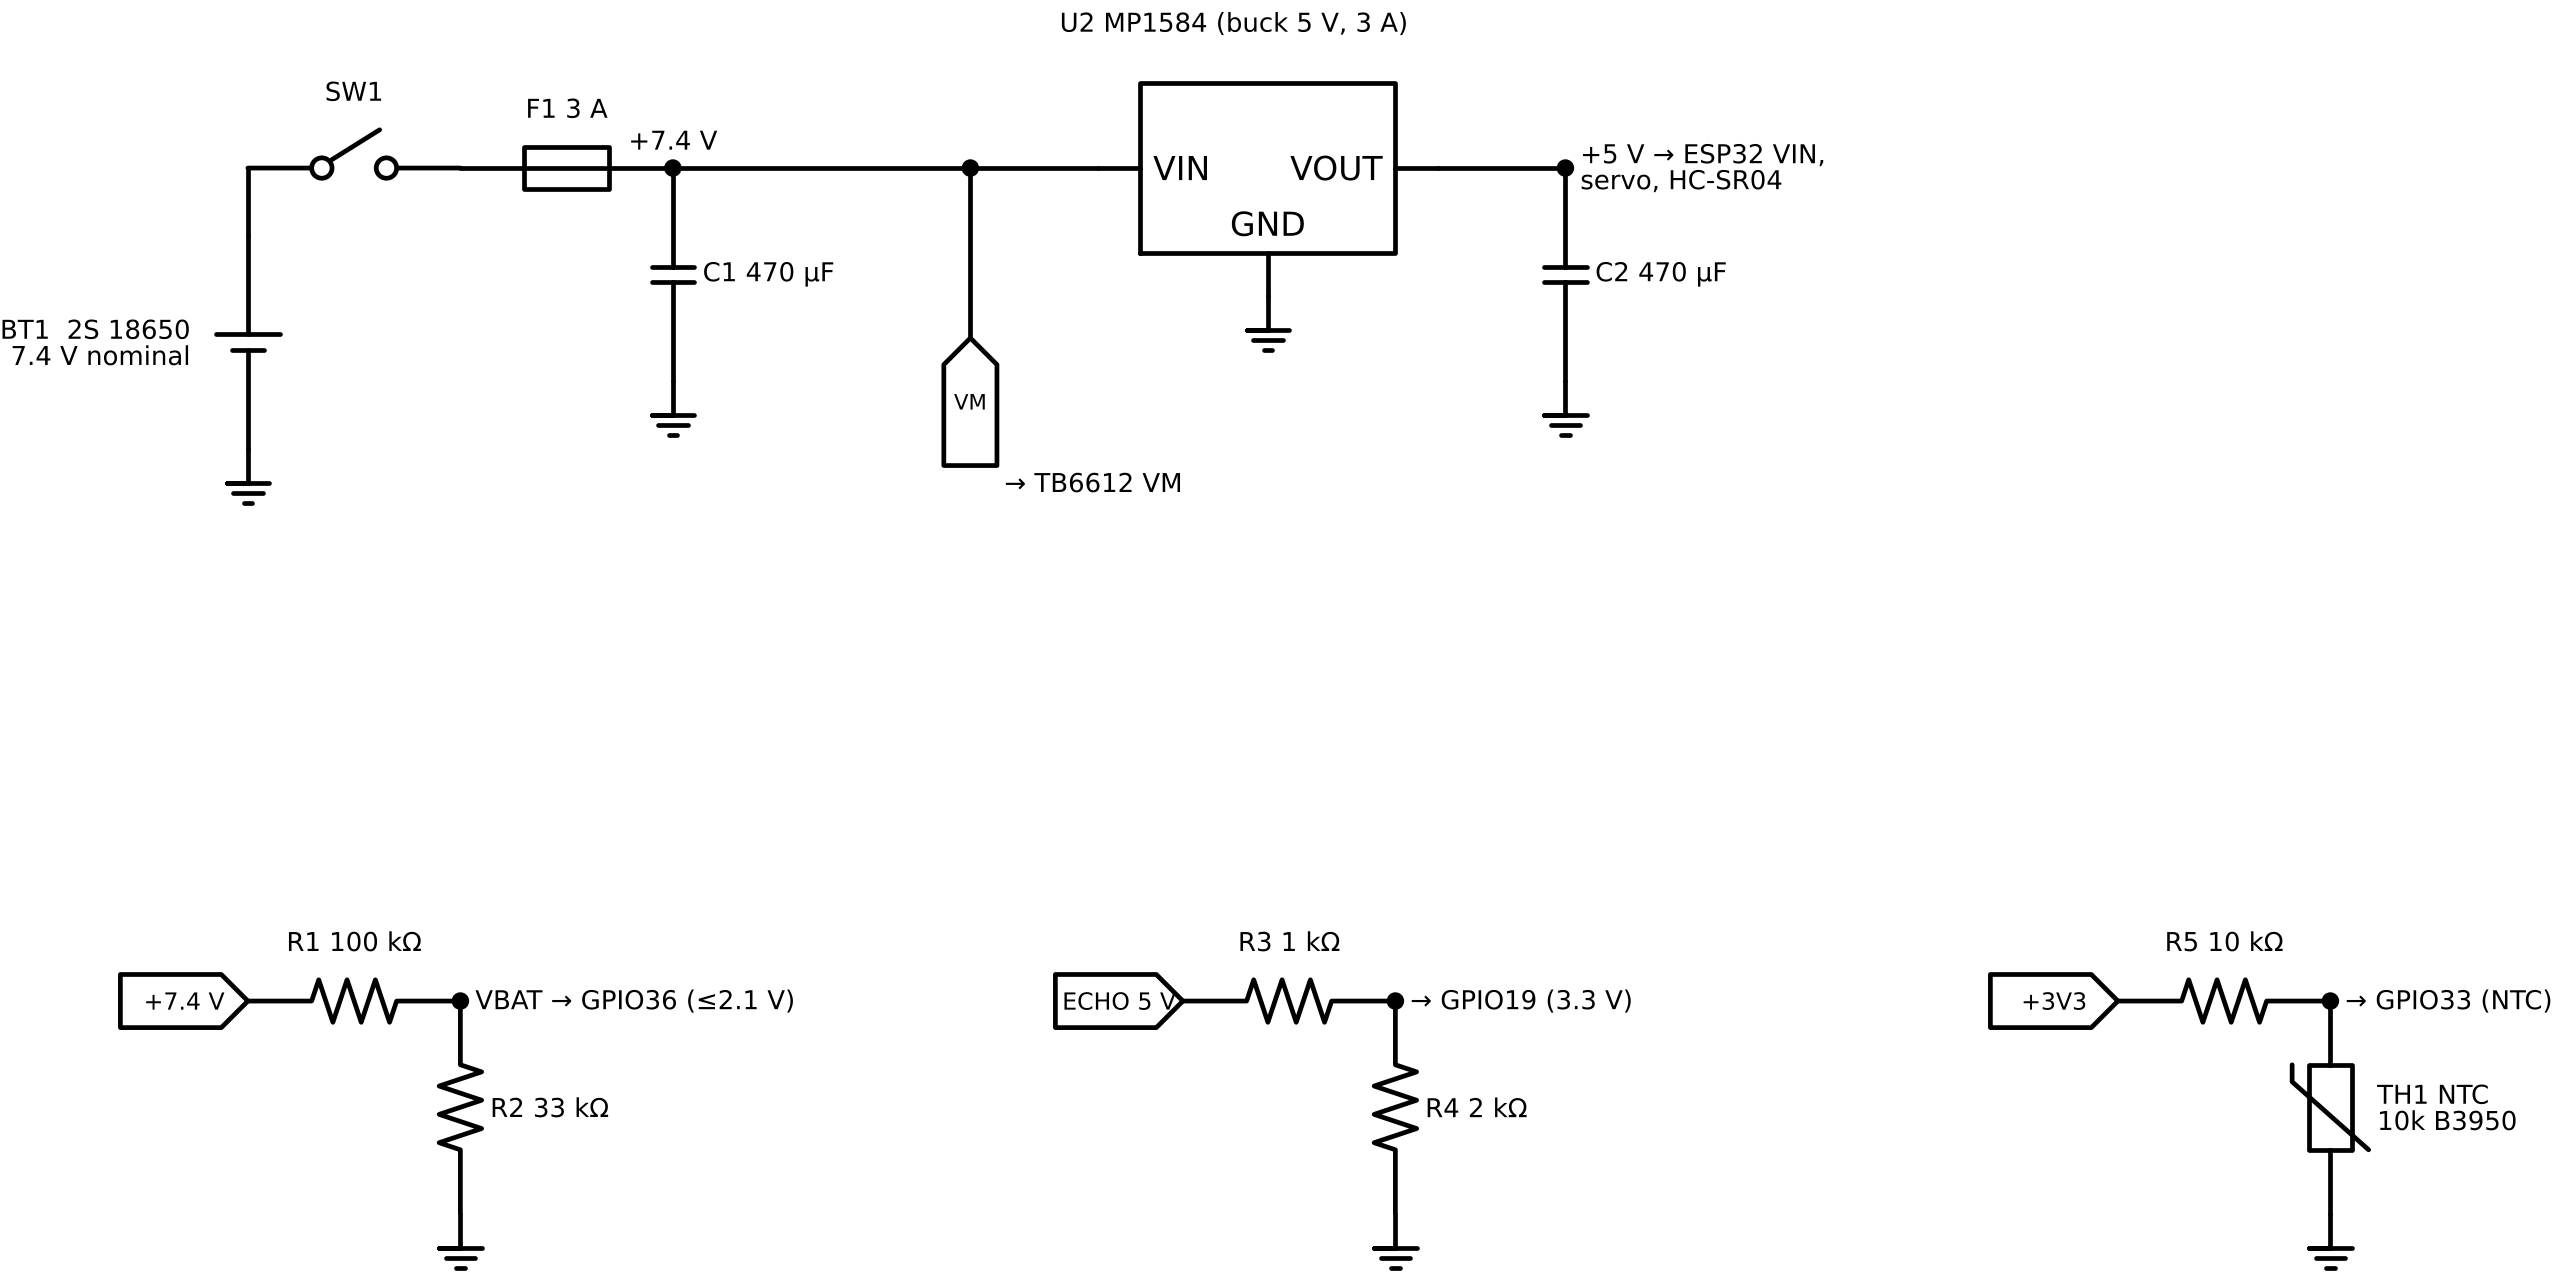
\includegraphics[width=0.82\textwidth]{fig/esquematico.png}
\caption{Etapa de potencia y divisores de tensión (batería, ECHO del ultrasonido y termistor).}\label{fig:pot}
\end{figure*}

\begin{table}[!t]
\caption{Asignación de pines del ESP32}\label{tab:pines}
\centering\scriptsize
\begin{tabular}{@{}lll@{}}
\toprule
\textbf{Elemento} & \textbf{Terminal} & \textbf{ESP32}\\
\midrule
TB6612 canal A (izq.) & PWMA / AIN1 / AIN2 & GPIO 25 / 26 / 27\\
TB6612 canal B (der.) & PWMB / BIN1 / BIN2 & GPIO 14 / 16 / 32\\
TB6612 & STBY & GPIO 13\\
QMC5883L y TCS34725 & SDA / SCL & GPIO 21 / 22\\
TCS34725 & LED & GPIO 4\\
HC-SR04 & TRIG / ECHO (1k/2k) & GPIO 18 / 19\\
Servo SG90 & señal & GPIO 23\\
TCRT5000 izq./centro/der. & D0 & GPIO 34 / 35 / 39\\
Batería (100k/33k) & divisor & GPIO 36\\
Termistor NTC (10k) & divisor & GPIO 33\\
LED de estado & ánodo & GPIO 2\\
\bottomrule
\end{tabular}
\end{table}

Los divisores se calcularon así: para la batería, $V_o=8{,}4\cdot33/133=2{,}08$\,V, dentro del rango del ADC con atenuación de 11\,dB; para el ECHO del ultrasonido, $5\cdot2/3=3{,}33$\,V, compatible con la entrada del ESP32; y para el NTC a 25\,°C, $V_o=3{,}3\cdot10/20=1{,}65$\,V, en la zona más lineal del ADC. El PWM de los motores es de 20\,kHz (inaudible) y se limita al 80\,\% del ciclo útil, unos 5,9\,V efectivos sobre motores de 6\,V. Con un consumo estimado de 1,3\,A, la batería de 2,6\,Ah da una autonomía de unas $2{,}6\cdot0{,}8/1{,}3\approx1{,}6$\,h.

\begin{figure*}[!t]
\centering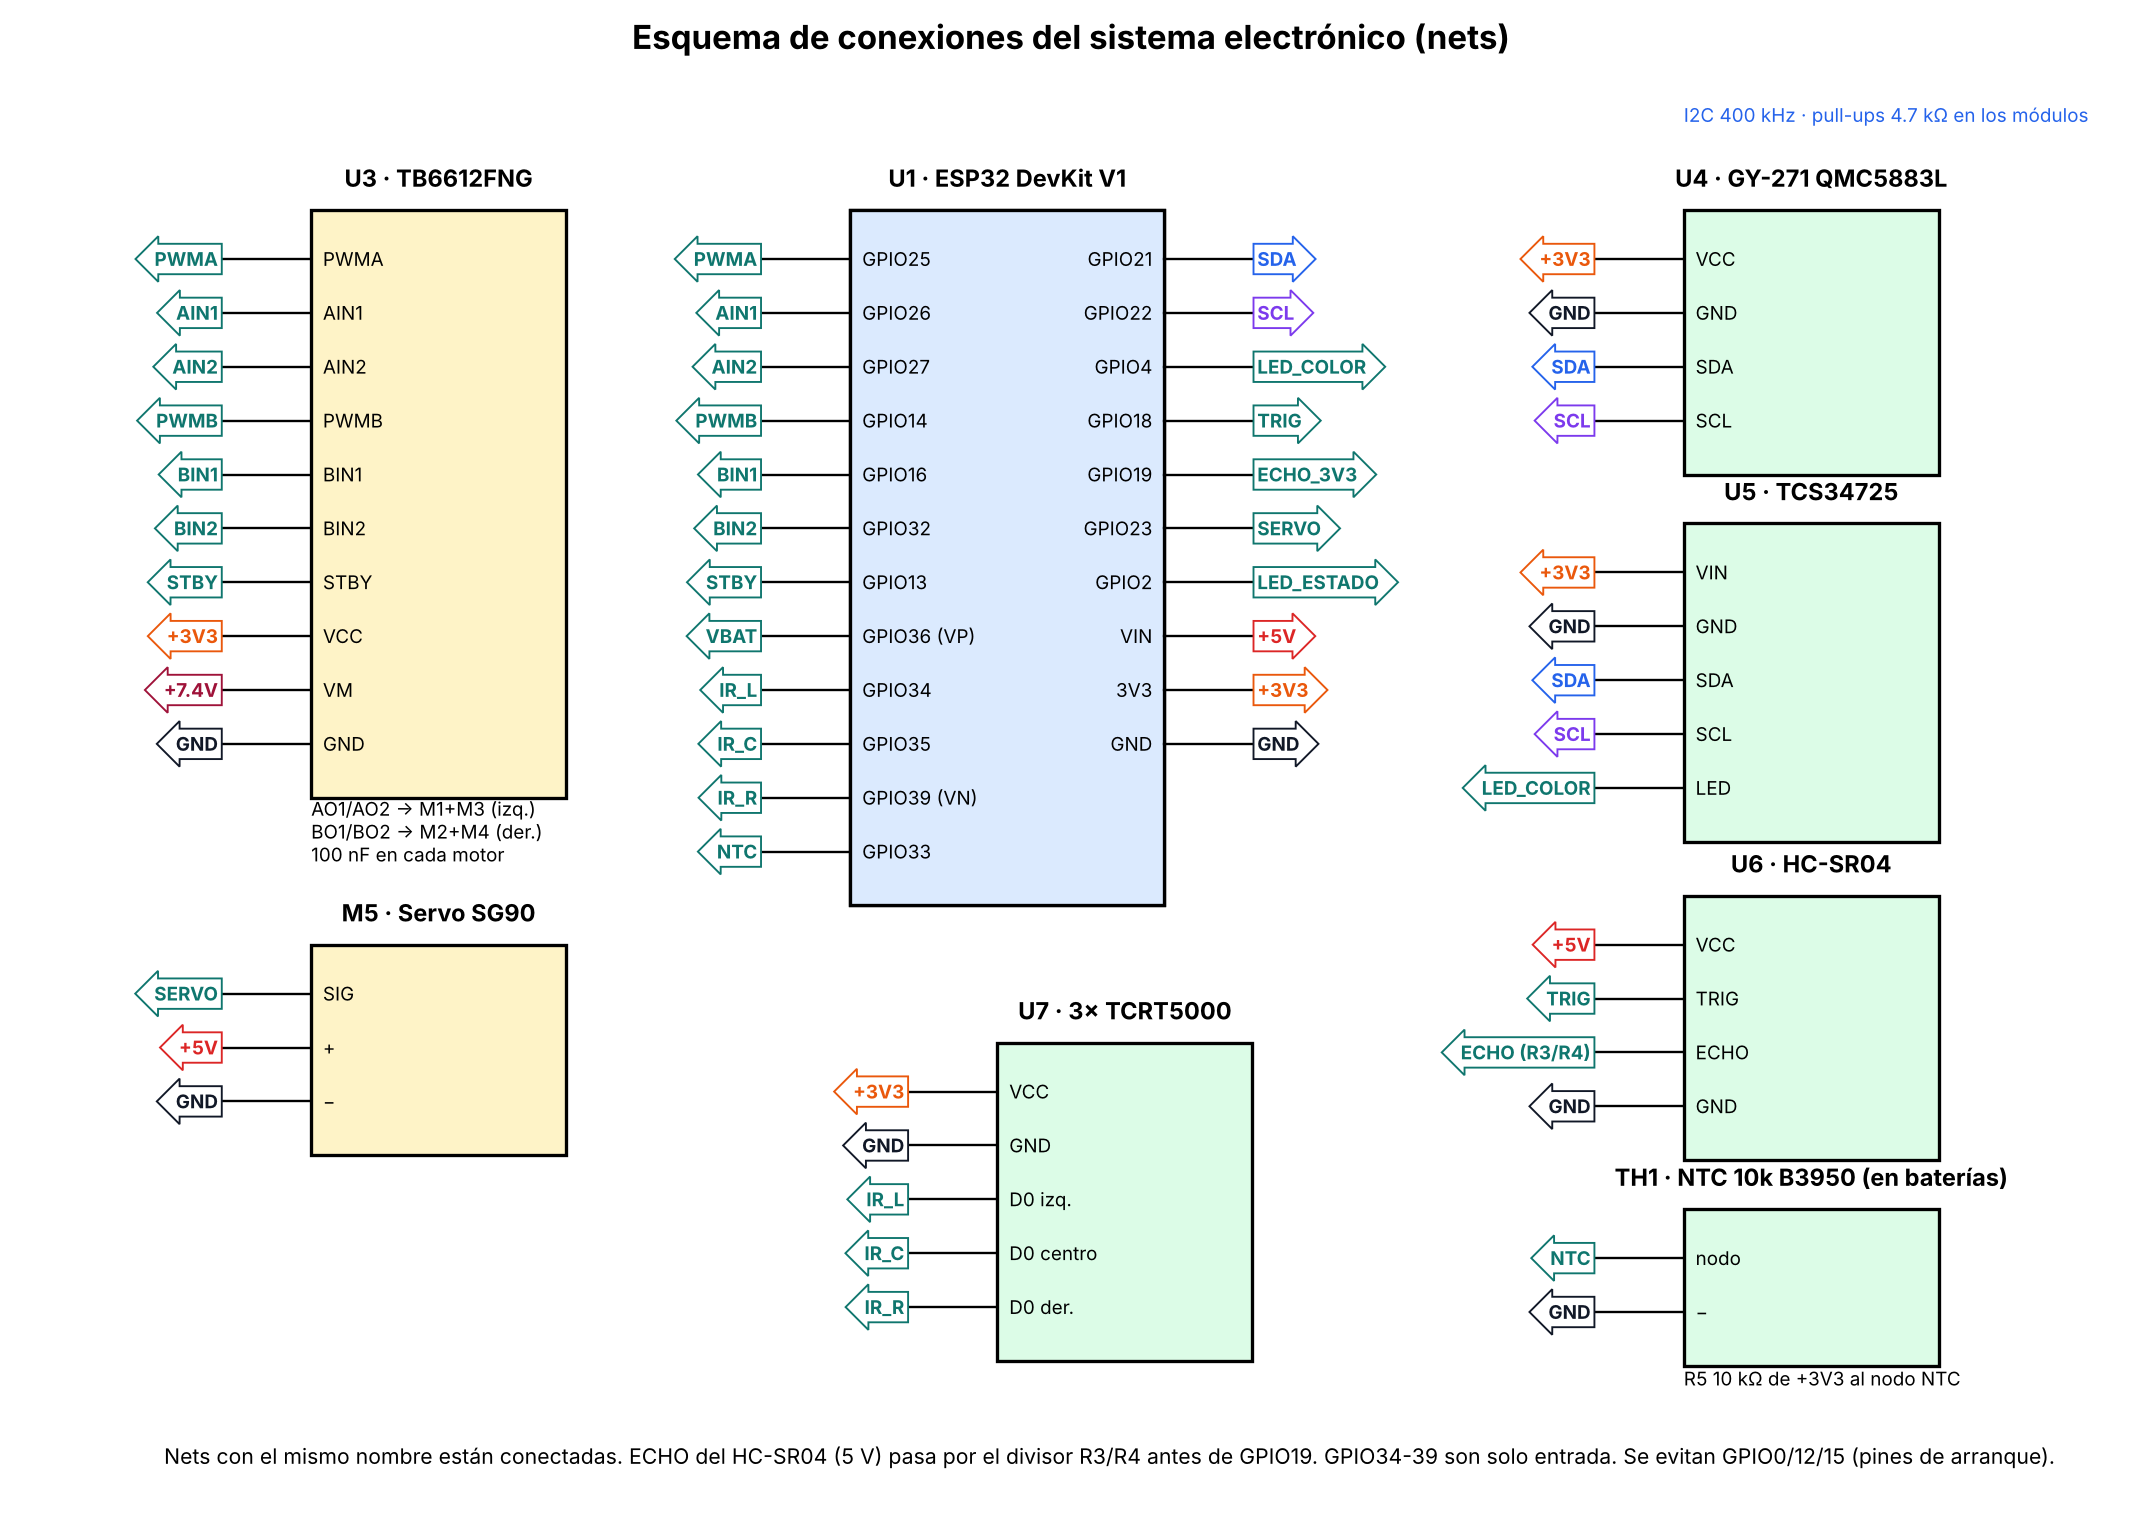
\includegraphics[width=0.86\textwidth]{fig/esquematico_esp32.png}
\caption{Conexiones del ESP32 con cada módulo (las redes con el mismo nombre están unidas).}\label{fig:nets}
\end{figure*}

\subsection{Firmware}
El firmware está organizado en un archivo por módulo (Tabla~\ref{tab:fw}); todos los parámetros están en \texttt{config.h}. En cada ciclo de 50\,ms el programa lee la brújula, los sensores de línea, la batería, el termistor, el ultrasonido y el color; aplica la protección térmica y ejecuta el modo activo.

\begin{table}[!t]
\caption{Estructura del firmware}\label{tab:fw}
\centering\scriptsize
\begin{tabularx}{\columnwidth}{@{}l>{\raggedright\arraybackslash}X@{}}
\toprule
\textbf{Archivo} & \textbf{Responsabilidad}\\
\midrule
\texttt{config.h} & Pines, umbrales, ganancias y red.\\
\texttt{motors.h} & PWM LEDC, mezcla diferencial y freno activo.\\
\texttt{compass.h} & QMC5883L, calibración en memoria no volátil, filtro vectorial.\\
\texttt{color\_sensor.h} & TCS34725, clasificación y anti-rebote de 3 lecturas.\\
\texttt{sensors.h} & Ultrasonido (mediana de 3), servo, línea, batería y NTC.\\
\texttt{robot\_esp32.ino} & Lazo de 20\,Hz, máquina de estados, API y ESP-NOW.\\
\texttt{control\_remoto.ino} & Joystick y botones \ra\ paquete ESP-NOW a 20\,Hz.\\
\texttt{pruebas\_modulos.ino} & Menú serie para probar cada módulo en el montaje.\\
\bottomrule
\end{tabularx}
\end{table}

\textbf{Brújula.} El filtro paso-bajo se aplica al vector unitario $(\hat m_x,\hat m_y)/\|\hat m\|$ y no al ángulo, para evitar el salto de $359^\circ$ a $0^\circ$. La calibración gira el robot 8\,s en el sitio y guarda offsets y escalas en memoria no volátil.

\textbf{Color.} Se clasifica por vecino más cercano en $(\tilde r,\tilde g,\tilde b,\log_{10}C)$ con el brillo ponderado a 0,25, y un cambio de sección se acepta tras tres lecturas iguales (unos 150\,ms). En la sección negra la línea guía es blanca, así que el color detectado invierte la polaridad de los TCRT5000.

\textbf{Modo autónomo.} La Fig.~\ref{fig:estados} muestra la máquina de estados. En \textsc{Seguir} el robot sigue la línea con $w^\ast=0{,}45\,e$ y la dirección deseada acompaña la orientación de la pista. Si pierde la línea, mantiene el rumbo con la brújula durante 0,8\,s y luego la busca en una espiral que se abre con el tiempo. Si el ultrasonido mide menos de 30\,cm:
\begin{enumerate}
\item frena y guarda el rumbo $h_0$;
\item escanea a 160$^\circ$ y a 20$^\circ$ con el servo y elige el lado más libre $s=\pm1$;
\item gira a $h_0+60^\circ s$ y avanza 0,7\,s;
\item rodea el obstáculo en arco ($w^\ast=-0{,}13\,s$) hasta encontrar la línea;
\item avanza 0,3\,s para quedar sobre la línea y pivota hacia el lado $s$ hasta que el sensor central la cruza con un rumbo a menos de $100^\circ$ de $h_0$, lo que asegura retomar la pista en el sentido original.
\end{enumerate}

\begin{figure}[!t]
\centering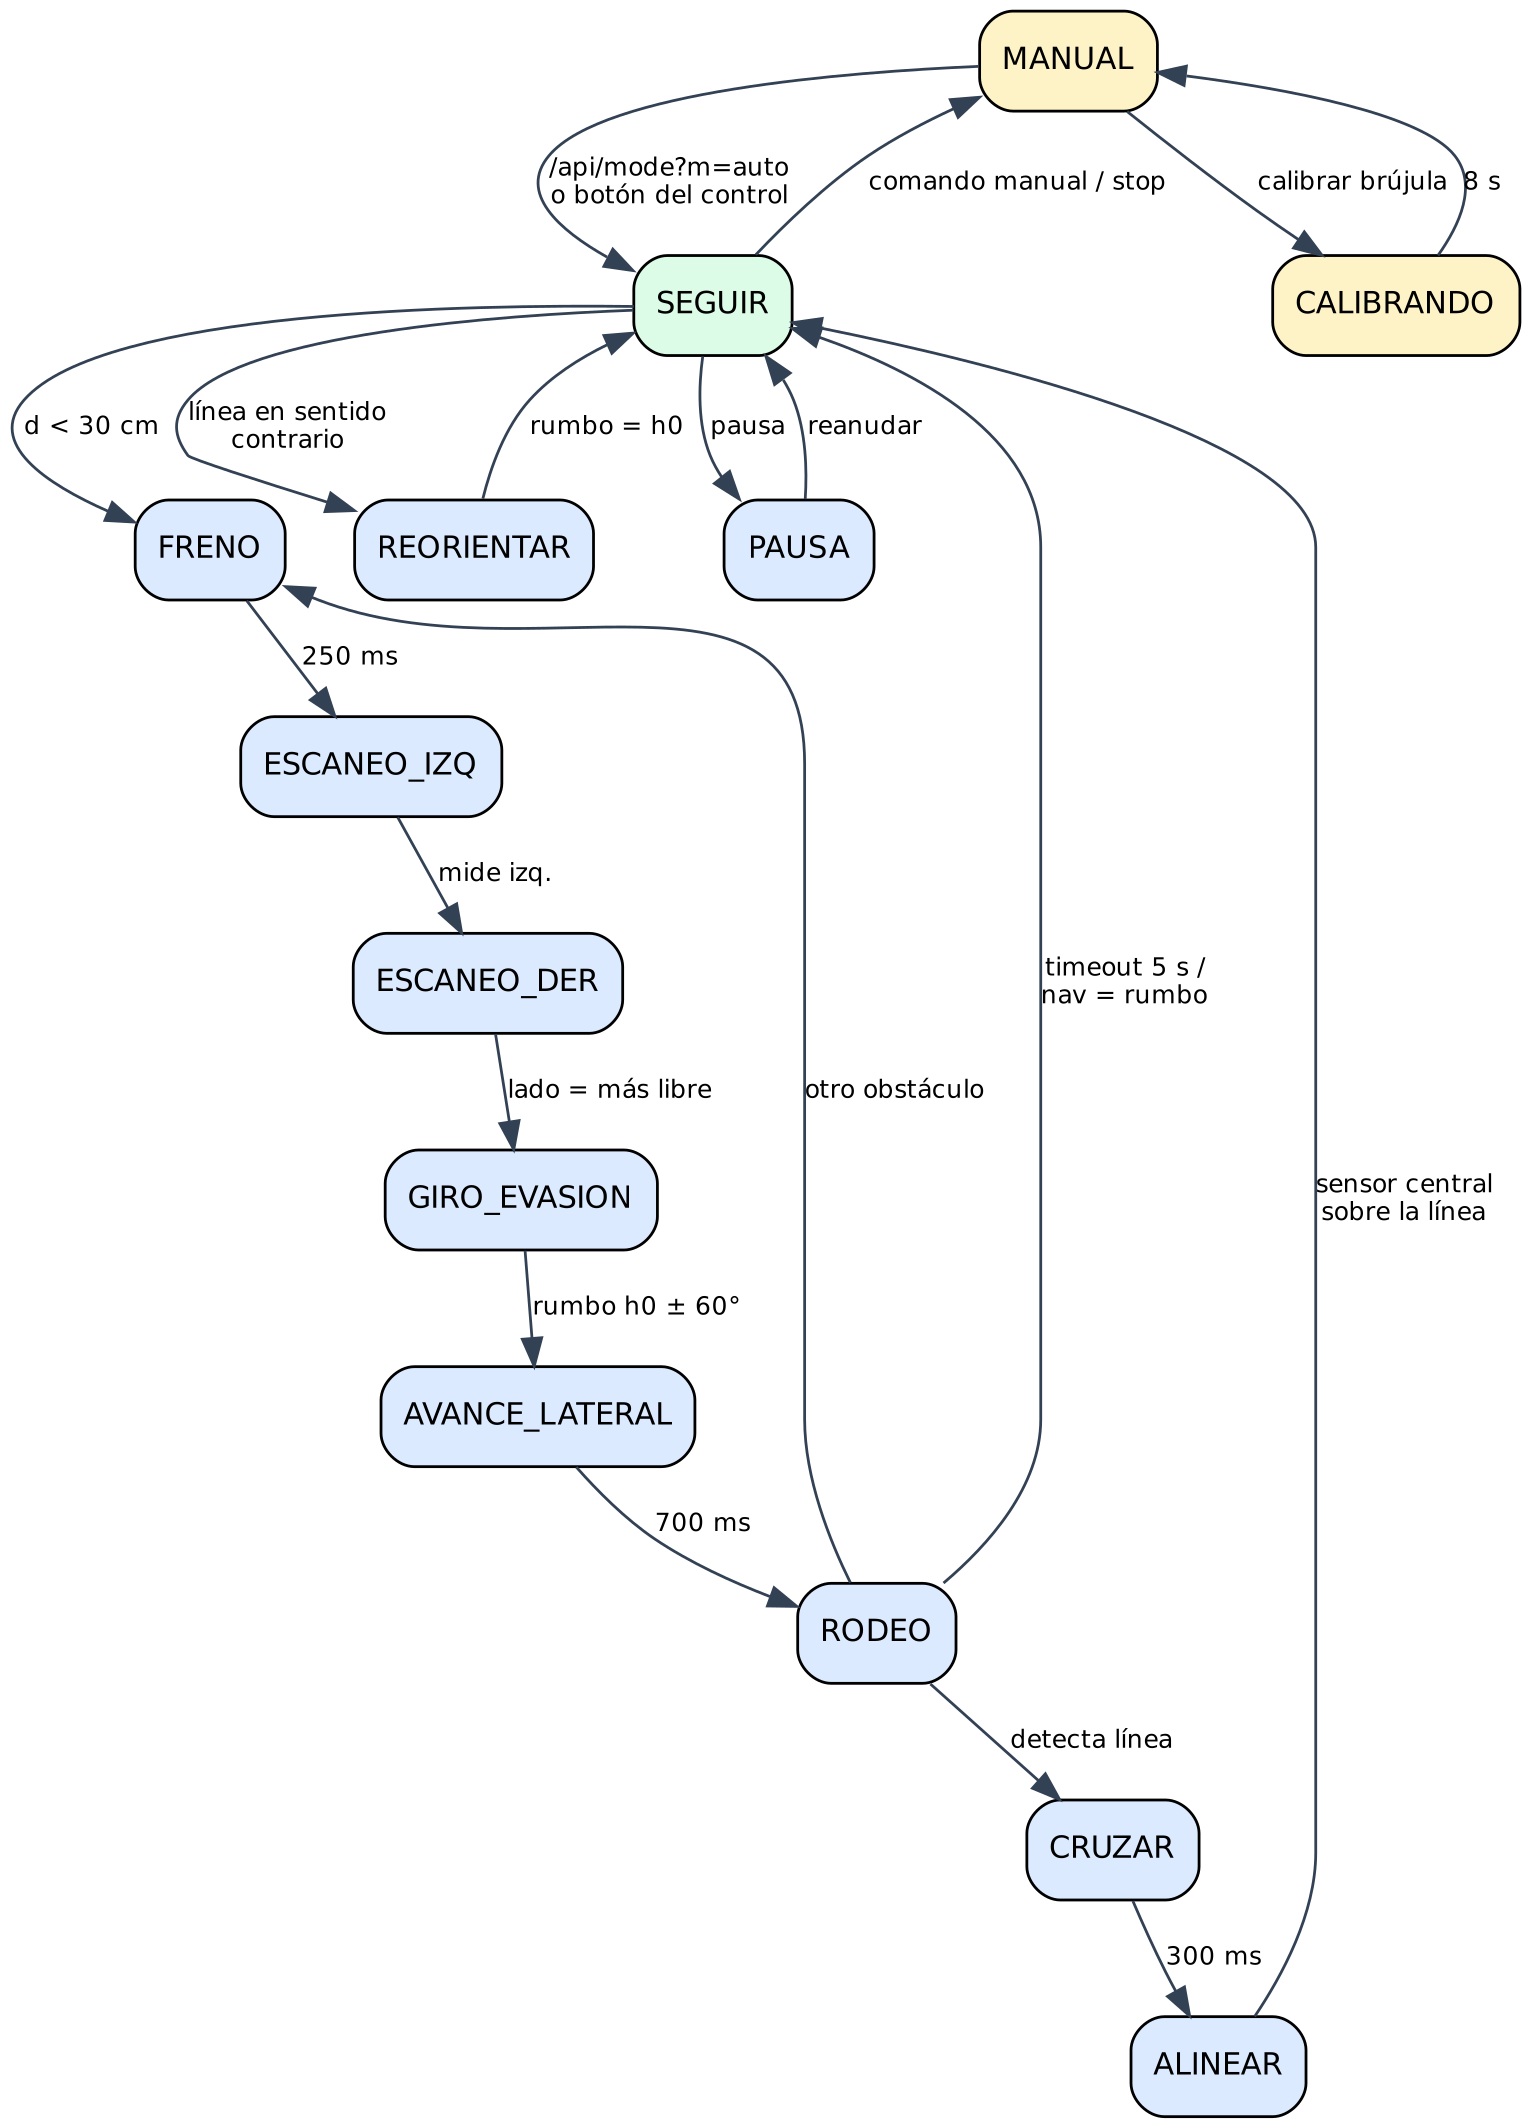
\includegraphics[width=\columnwidth]{fig/maquina_estados.png}
\caption{Máquina de estados del firmware.}\label{fig:estados}
\end{figure}

\textbf{Protección térmica.} El NTC se lee con un promedio de cuatro muestras y un filtro paso-bajo. A 45\,°C se emite un aviso; a 55\,°C se detienen los motores, se pasa a modo manual con velocidad limitada al 40\,\% y se bloquea el modo autónomo hasta bajar de 40\,°C (histéresis de 5\,°C). Si la lectura indica circuito abierto o corto, la protección se desactiva y la app lo reporta.

\textbf{Seguridad.} Los comandos manuales son pulsos con duración, así que si se pierde la conexión el robot se detiene; además se bloquea el avance si hay un obstáculo a menos de 12\,cm.

\subsection{Comunicación y aplicación}
El ESP32 crea la red \texttt{ROBOT-ESP32} (192.168.4.1) y escucha ESP-NOW en el mismo canal. La API (Tabla~\ref{tab:api}) entrega toda la telemetría en JSON: rumbo actual y deseado, error, distancia, color, valores RGBC, sensores de línea, motores, batería, temperatura, estado y último evento.

\begin{table}[!t]
\caption{API HTTP del robot (igual en el ESP32 y en el simulador)}\label{tab:api}
\centering\scriptsize
\begin{tabularx}{\columnwidth}{@{}l>{\raggedright\arraybackslash}X@{}}
\toprule
\textbf{Endpoint} & \textbf{Acción}\\
\midrule
\texttt{/api/state} & Telemetría completa en JSON.\\
\texttt{/api/cmd?move=\ldots} & Movimiento manual por pulsos (\texttt{forward}, \texttt{backward}, \texttt{left}, \texttt{right}, \texttt{stop}).\\
\texttt{/api/mode?m=\ldots} & \texttt{auto}, \texttt{manual}, \texttt{pausa}, \texttt{reanudar}; navegación por línea o por rumbo.\\
\texttt{/api/heading?deg=\ldots} & Dirección polar deseada (absoluta o relativa).\\
\texttt{/api/calibrate} & Calibración de brújula o de un color.\\
\bottomrule
\end{tabularx}
\end{table}

La aplicación Streamlit (Fig.~\ref{fig:app}) se actualiza cada 0,5\,s y muestra la brújula polar con la dirección actual y la deseada, la pista en el simulador, los sensores, los motores, la batería, la temperatura y los eventos. Los comandos de voz se graban en el navegador, se reconocen en español y un intérprete los traduce a la API («arriba», «gira 45 grados a la derecha», «rumbo 90», «modo automático», «detente»). J.A.R.V.I.S. recibe la telemetría actual con cada pregunta y responde con los valores en tiempo real usando la API de Claude; sin conexión responde con un motor de reglas local.

\begin{figure*}[!t]
\centering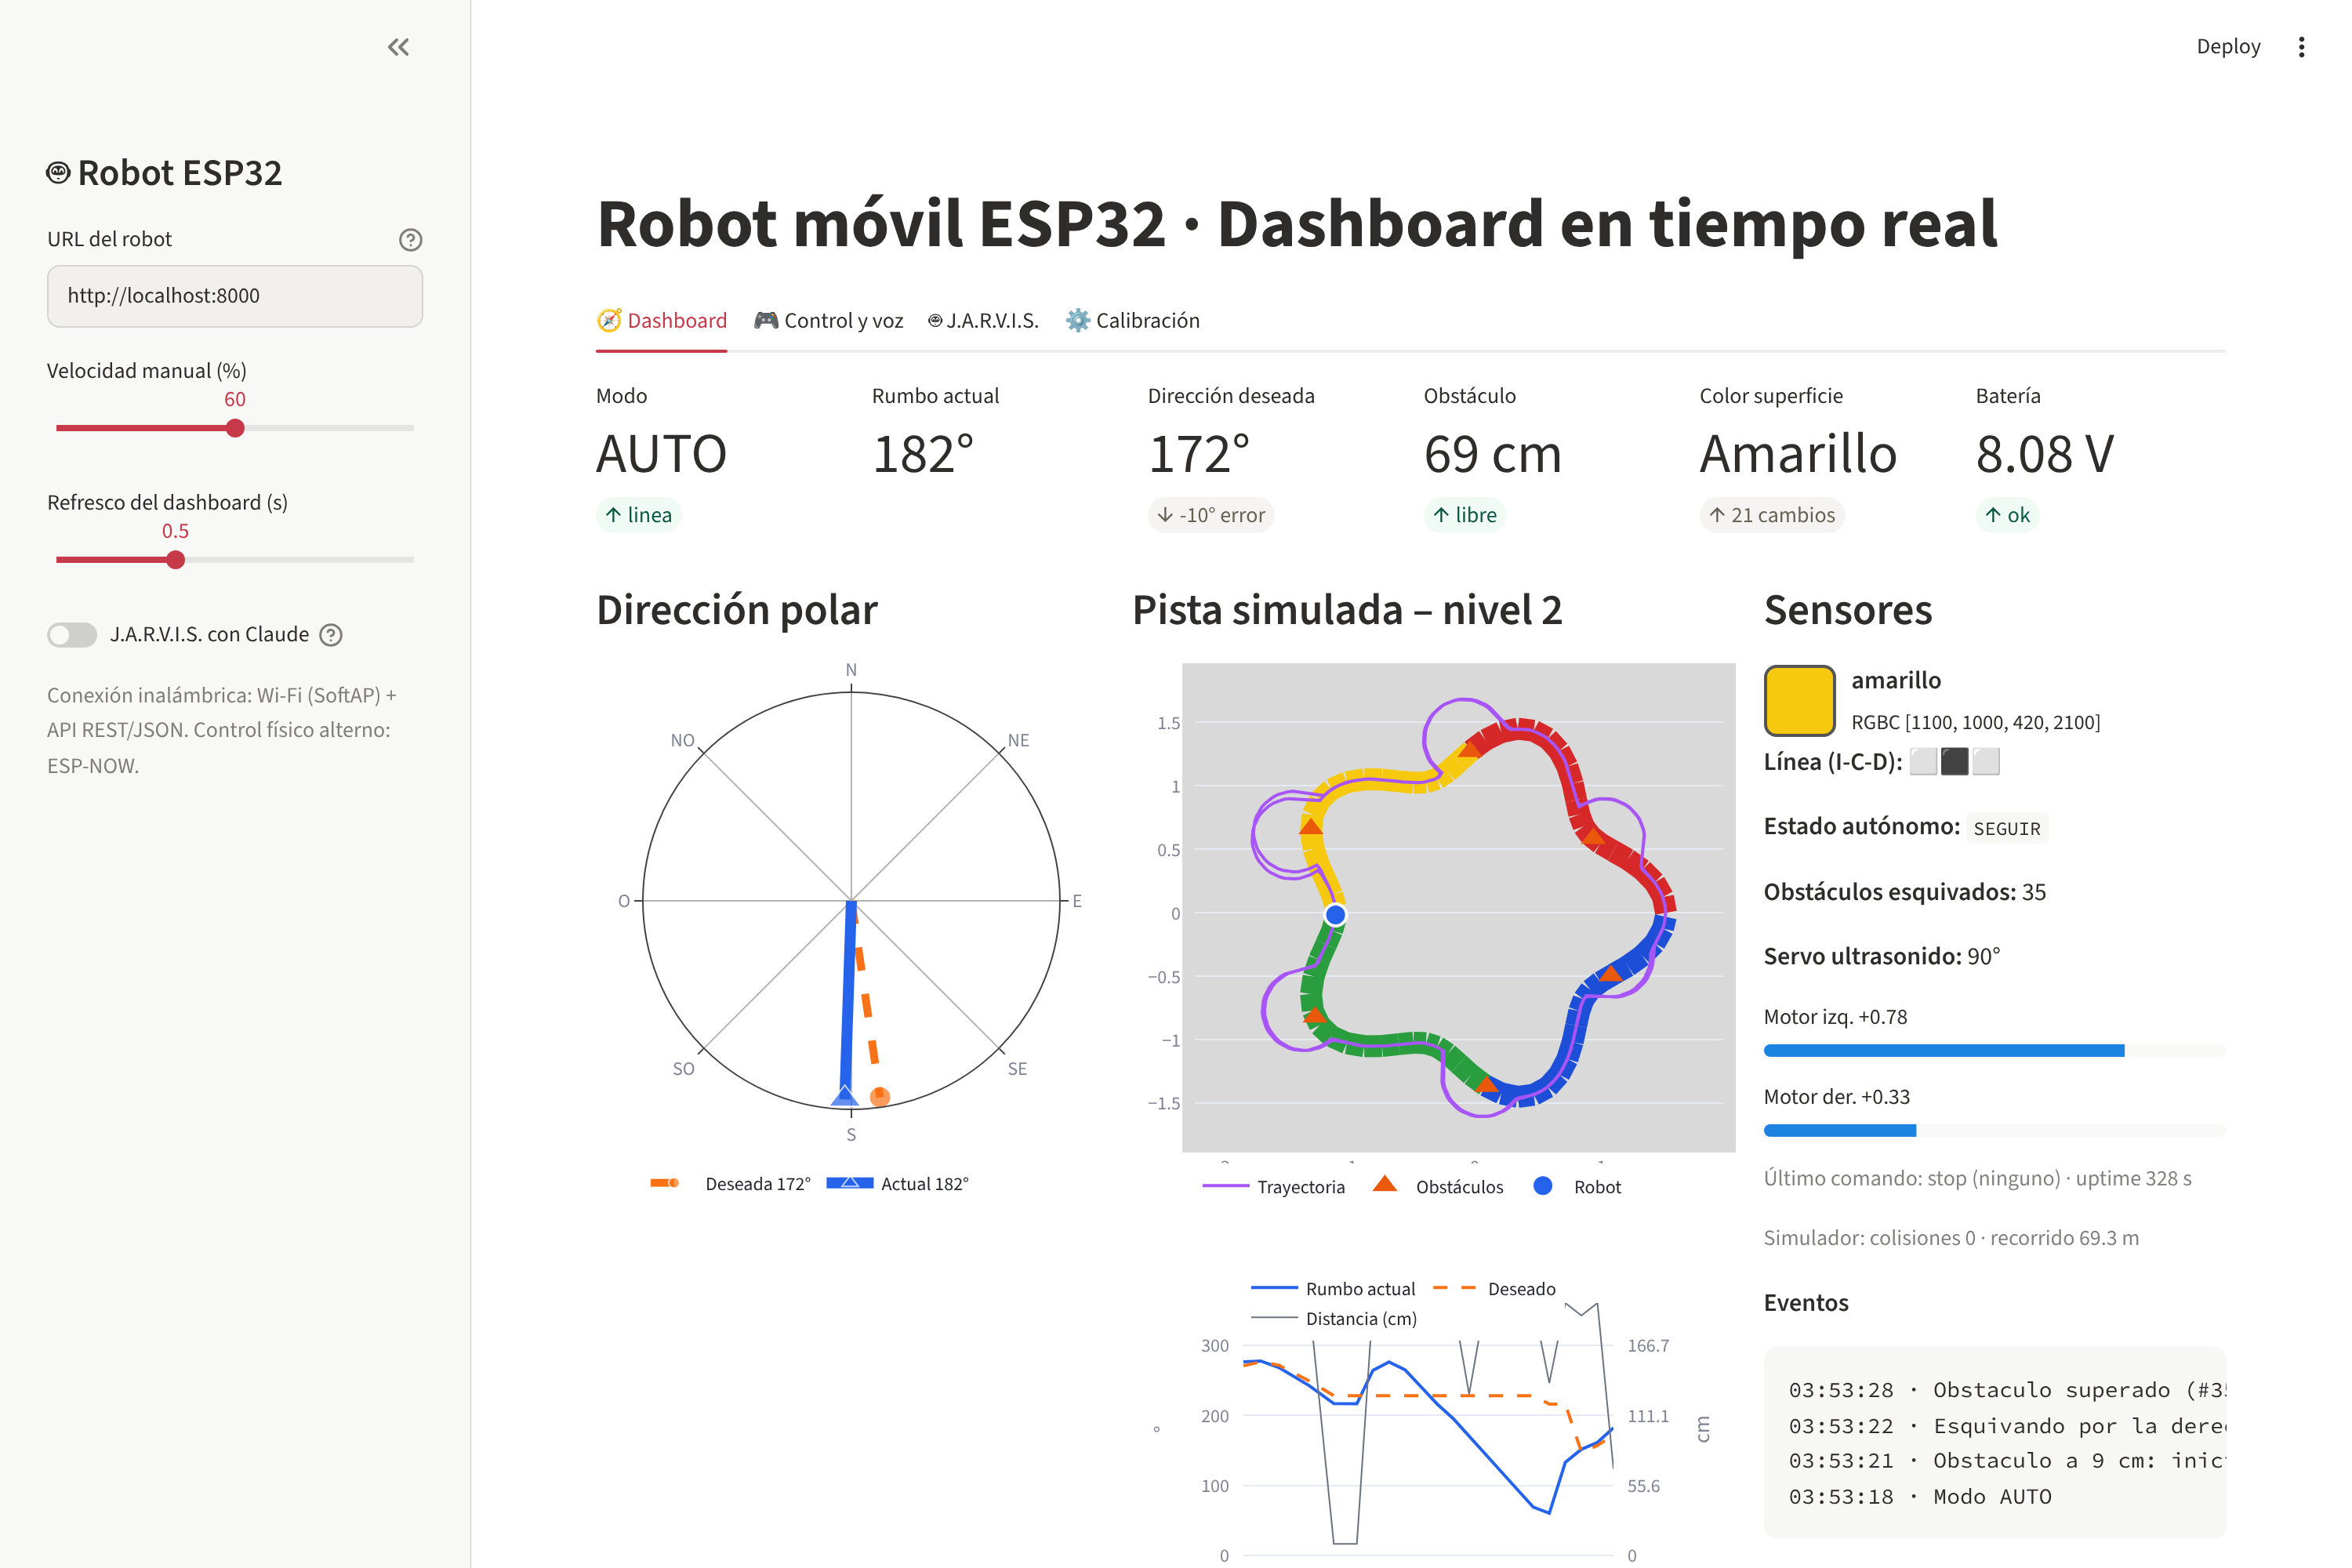
\includegraphics[width=0.85\textwidth]{fig/app_dashboard.png}
\caption{Tablero Streamlit conectado al gemelo digital.}\label{fig:app}
\end{figure*}

\subsection{Gemelo digital y pistas}
El simulador implementa la cinemática diferencial, la brújula con ruido ($\sigma=0{,}8^\circ$), un ultrasonido con haz de $\pm15^\circ$, los tres sensores de línea, el sensor de color por sección y un modelo térmico de primer orden del paquete de baterías. Como expone la misma API que el ESP32, la aplicación y el chatbot funcionan igual con el robot real o con el simulador.

Las pistas se diseñaron para dibujarse sobre pliegos de $70\times100$\,cm: solo la línea guía de 19\,mm sobre una franja de color, con curvas de radio $\geq20$\,cm y obstáculos separados unos 70\,cm (Fig.~\ref{fig:pistas}). Para cada una se generó un plano a escala y una tabla con las coordenadas de la línea cada 20\,cm.

\begin{figure}[!t]
\centering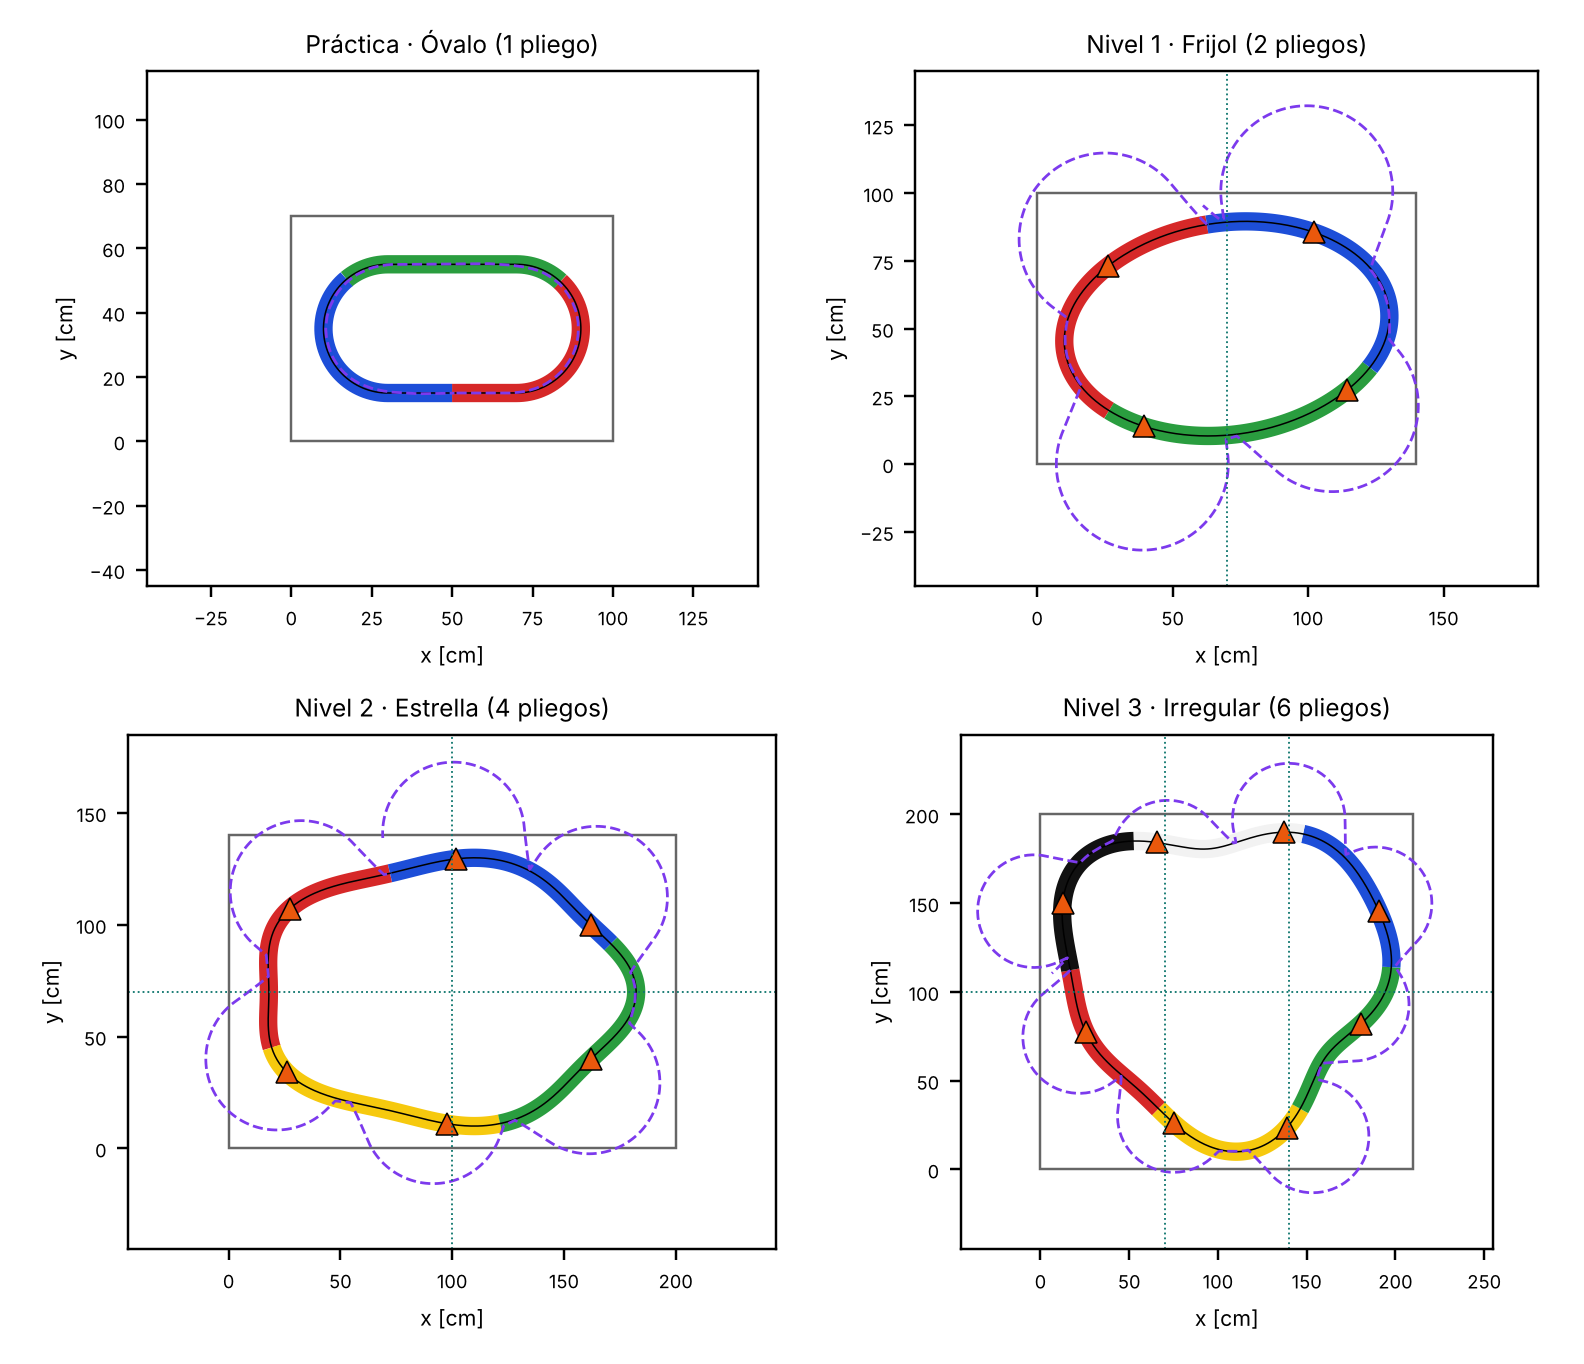
\includegraphics[width=\columnwidth]{fig/simulacion_pliegos.png}
\caption{Pistas sobre pliegos (líneas punteadas: uniones) y primera vuelta simulada (morado). Los triángulos son los conos.}\label{fig:pistas}
\end{figure}

\subsection{Montaje y pruebas por módulo}\label{sec:montaje}
El montaje sigue el orden mecánica\ra potencia\ra control\ra sensores, y cada módulo se prueba apenas se conecta con el programa \texttt{pruebas\_modulos.ino} (Tabla~\ref{tab:pruebas}). Antes de conectar cargas, el regulador se ajusta a 5,0\,V con el multímetro.

\begin{table}[!t]
\caption{Programa de pruebas por módulo (monitor serie, 115200 baudios)}\label{tab:pruebas}
\centering\scriptsize
\begin{tabularx}{\columnwidth}{@{}c>{\raggedright\arraybackslash}X@{}}
\toprule
\textbf{Tecla} & \textbf{Prueba y criterio}\\
\midrule
1 & Escáner I$^2$C: deben aparecer 0x0D y 0x29.\\
2 & Motores con el robot levantado: cada lado adelante y atrás.\\
3 & Sensores de línea: 1 sobre la cinta y 0 sobre el piso.\\
4 & Brújula: rumbo 0--360$^\circ$ sin saltos al girar.\\
5 & Color: valores RGBC distinguibles en los seis colores.\\
6 & Ultrasonido y servo: barrido 20--160$^\circ$; mano a 20\,cm.\\
7 & Batería y termistor: voltaje $\pm0{,}1$\,V del multímetro y 20--30\,°C.\\
8 & Todo en vivo cada 250\,ms.\\
\bottomrule
\end{tabularx}
\end{table}

\section{Preguntas para la discusión}
\begin{enumerate}[label=\textbf{\arabic*)},leftmargin=1.6em]
\item \textbf{¿Por qué la brújula va en un mástil?} Los imanes de los motores y los tornillos de acero deforman el campo local. A unos 125\,mm la distorsión es pequeña y lo que queda se corrige con la calibración de hierro duro y blando.
\item \textbf{¿Por qué se usa cromaticidad y no los valores RGB directos?} Los valores absolutos cambian con la iluminación y la altura del sensor. Al dividir por $R+G+B$ queda solo el tono, y el brillo se usa aparte para separar blanco de negro.
\item \textbf{¿Por qué el termistor va en GPIO33?} El ADC2 del ESP32 lo usa el radio Wi-Fi y no se puede leer con la red activa. GPIO33 es del ADC1; para liberarlo, BIN1 se movió a GPIO16, que no es pin de arranque.
\item \textbf{¿Por qué el robot pivota hacia el lado de la evasión al retomar la línea?} Al volver, el robot cruza la línea en diagonal. Girando hacia el lado por el que esquivó, el primer cruce del sensor central corresponde al sentido de avance; el chequeo con $h_0$ descarta el sentido contrario en curvas cerradas.
\item \textbf{¿Por qué en la sección negra la línea es blanca?} Los TCRT5000 detectan contraste. Sobre negro una cinta negra no se distingue, así que se usa blanca y el firmware invierte la lectura cuando el sensor de color detecta negro.
\item \textbf{¿Por qué los conos deben medir al menos 18\,cm?} El ultrasonido está a unos 110\,mm del piso y su haz se abre unos $\pm15^\circ$. Un obstáculo más bajo puede quedar por debajo del haz.
\item \textbf{¿Por qué validar en un gemelo digital?} Permite probar la lógica completa antes de tener el hardware y repetir miles de maniobras. Así se encontró un error de alineación que habría sido difícil de diagnosticar en la pista real (Sección~\ref{sec:resultados}).
\end{enumerate}

\section{Análisis de resultados}\label{sec:resultados}
\subsection{Simulación en las pistas sobre pliegos}
La Tabla~\ref{tab:sim} resume la simulación. La práctica no lleva cono porque en un solo pliego no hay suficiente recta para la maniobra. En 5 minutos continuos, las tres pistas de evaluación se recorrieron entre 5,8 y 10 veces, con 40, 44 y 46 evasiones y ninguna colisión. La mayor separación de la línea durante una evasión fue de 47--48\,cm, por lo que debe quedar piso libre alrededor del papel.

\begin{table}[!t]
\caption{Resultados en el gemelo digital (5 min de recorrido)}\label{tab:sim}
\centering\scriptsize
\setlength{\tabcolsep}{3.2pt}
\begin{tabular}{@{}lcccccc@{}}
\toprule
\textbf{Pista} & \textbf{Pliegos} & \textbf{Línea} & \textbf{Conos} & \textbf{1.ª vuelta} & \textbf{Evasiones} & \textbf{Desvío}\\
 & & [m] & & [s] & / colisiones & máx. [cm]\\
\midrule
Práctica & 1 & 2,06 & 0 & 7 & 0 / 0 & 1\\
Nivel 1 & 2 & 3,15 & 4 & 32 & 40 / 0 & 47\\
Nivel 2 & 4 & 4,52 & 6 & 39 & 44 / 0 & 47\\
Nivel 3 & 6 & 5,80 & 8 & 54 & 46 / 0 & 48\\
\bottomrule
\end{tabular}
\end{table}

\subsection{Error encontrado en la alineación}
En la primera versión, el estado \textsc{Alinear} solo aceptaba el cruce de la línea después de 0,25\,s. En las curvas de la estrella el sensor central cruzaba la línea antes de ese tiempo; el robot seguía girando, daba una vuelta casi completa y quedaba en sentido contrario, por lo que volvía a encontrar el mismo cono. Se cambió el criterio: el cruce se acepta cuando el sensor central ya salió de la línea y el rumbo está a menos de $100^\circ$ de $h_0$. Con esta corrección todas las pistas se completan, y el caso quedó cubierto por las pruebas automáticas (31 en total).

\subsection{Limitaciones}
Los resultados dependen del modelo del simulador: el ancho de vía, la velocidad máxima y la posición de los sensores se estimaron, y no se modelan el deslizamiento de las ruedas ni el ruido de los sensores de línea. El firmware se verificó por compilación y en simulación, pero aún falta probarlo en el robot físico. Las ganancias ($K_l$, el arco de evasión y la velocidad) deberán ajustarse con el robot real a partir de la pista de práctica.

\section{Conclusiones}
\begin{enumerate}
\item La arquitectura centralizada en el ESP32, con un lazo de 20\,Hz y una API REST única, permite que la aplicación, el chatbot y el control remoto usen los mismos datos en tiempo real.
\item Separar los dominios de potencia y montar la brújula en un mástil no metálico son las decisiones que más afectan la confiabilidad del magnetómetro y del microcontrolador.
\item La cromaticidad normalizada del TCS34725, con LED propio y faldón, permite clasificar seis colores con un algoritmo simple y calibrable en la pista.
\item El gemelo digital con la misma API del firmware permitió desarrollar la aplicación y validar la lógica autónoma antes del montaje, y reveló un error de alineación que habría hecho que el robot recorriera la pista al revés.
\item Por el espacio que requiere la evasión, cada pista de evaluación necesita 2, 4 o 6 pliegos; un solo pliego sirve como pista de práctica para calibrar la línea y los colores.
\end{enumerate}

\begin{thebibliography}{9}\small
\bibitem{espressif} Espressif Systems, ``ESP32 Series Datasheet,'' v4.x, 2024.
\bibitem{qmc} QST Corporation, ``QMC5883L 3-Axis Magnetic Sensor,'' hoja de datos, rev. 1.0.
\bibitem{tcs} ams-OSRAM, ``TCS3472 Color Light-to-Digital Converter with IR Filter,'' hoja de datos.
\bibitem{tb} Toshiba, ``TB6612FNG Driver IC for Dual DC Motor,'' hoja de datos.
\bibitem{tcrt} Vishay, ``TCRT5000 Reflective Optical Sensor with Transistor Output,'' hoja de datos.
\bibitem{mps} Monolithic Power Systems, ``MP1584 3A, 1.5MHz, 28V Step-Down Converter,'' hoja de datos.
\bibitem{siegwart} R. Siegwart, I. Nourbakhsh, D. Scaramuzza, \emph{Introduction to Autonomous Mobile Robots}, 2.ª ed. MIT Press, 2011.
\bibitem{noaa} NOAA NCEI, ``Magnetic Field Calculators,'' 2026.
\bibitem{streamlit} Streamlit Inc., ``Streamlit documentation,'' 2026.
\end{thebibliography}

\section*{\centering Anexos}
{\raggedright\noindent\textbf{Anexo A.} Código completo en el repositorio \url{https://github.com/anaescobarj/seguidor_de_linea}: firmware (\texttt{firmware/}), aplicación y simulador (\texttt{app/}), CAD (\texttt{hardware/cad/}), pistas (\texttt{docs/pistas/}) y guía de montaje (\texttt{docs/MONTAJE.md}).\par}

{\raggedright\noindent\textbf{Anexo B. Programa principal del ESP32 (\texttt{robot\_esp32.ino})}\par}
\lstinputlisting{fig/anexo_robot_esp32.ino}

\end{document}
